\chapter{L'ERREUR DE CALIBRAGE}
\begin{spacing}{1.2}
	\minitoc
	\thispagestyle{MyStyle}
\end{spacing}
\newpage

%----------------------------------------------------------------------------------------
%Notion de caméras	
%----------------------------------------------------------------------------------------
\section{INTRODUCTION}

Le calibrage d'une caméra est essentiel pour garantir que les images capturées sont précises et fidèles à la réalité. Cependant, plusieurs facteurs peuvent affecter la précision des résultats obtenus par une caméra. Dans ce chapitre, nous examinerons les différentes sources d'erreurs de calibrage d'une caméra et comment elles peuvent être corriger.

\section{Les Sources d'Erreurs de Calibrage d'une Caméra}

 Les sourcesd'erreur les plus importants sont:

 \begin{itemize}
	\item \textbf{Distorsion de l’objectif } :  La distorsion de l’objectif peut entraîner des erreurs importantes dans le processus d’étalonnage de l’appareil photo. La distorsion se produit lorsque l’objectif projette le monde 3D sur le plan de l’image 2D, ce qui donne l’impression que les lignes droites sont incurvées. Les types courants de distorsion comprennent la distorsion radiale, qui provoque le gonflement de l’image vers l’extérieur ou vers l’intérieur, et la distorsion tangentielle, qui provoque l’inclinaison de l’image. Le calcul des coefficients de distorsion et leurs correction lors du calibrage aide à corriger ces erreurs  (Figure \ref{fig:Types de distorsion}). 
	
	\begin{figure}[h]
		\centering
		\fbox{
			\begin{minipage}{0.24\textwidth}
				\centering
				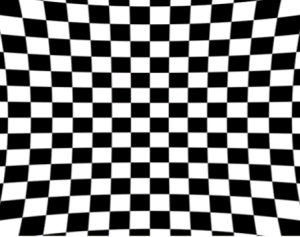
\includegraphics[width=\linewidth]{images/radialint}
				\subcaption{(a)}
			\end{minipage}\hfill
			\begin{minipage}{0.25\textwidth}
				\centering
				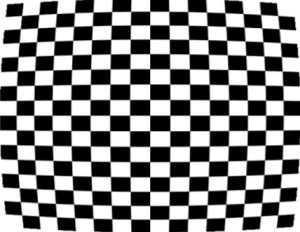
\includegraphics[width=\linewidth]{images/radialext}
				\subcaption{(b)}
			\end{minipage}\hfill
			\begin{minipage}{0.26\textwidth}
				\centering
				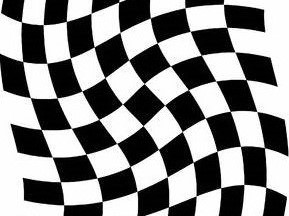
\includegraphics[width=\linewidth]{images/tang}
				\subcaption{(c)}
			\end{minipage}\hfill 
		}
		\caption[Types de distorsion]{(a)Distorsion radial intérieur, (b)Distorsion radial extérieur, (c) Distorsion tangentielle. Source :https://lens.google.com}
		\label{fig:Types de distorsion}
	\end{figure}
	
	\item \textbf{Résolution de l’image} : La résolution des images utilisées pour l’étalonnage de la caméra peut également affecter la précision des résultats. Les images haute résolution fournissent des informations plus détaillées sur le modèle d’étalonnage, ce qui peut conduire à des estimations plus précises de la matrice de projection de la caméra. Cependant, les images haute résolution nécessitent également plus de ressources de calcul et peuvent être plus difficiles à traiter.	\\
	
	\item \textbf{Placement de la caméra} : La position et l’orientation de la caméra peuvent également affecter la précision des résultats de l’étalonnage de la caméra. Les caméras doivent être placées à une distance suffisante du motif d’étalonnage pour s’assurer que la géométrie du motif est visible dans l’image. De plus, les caméras doivent être alignées parallèlement au motif pour minimiser la distorsion de perspective. \\
	
	\item \textbf{Qualité du modèle d’étalonnage} : la qualité du modèle d’étalonnage peut également affecter la précision des résultats d’étalonnage de la caméra. Les motifs d’étalonnage doivent être plats, rigides et avoir un contraste élevé pour garantir que la géométrie du motif est visible dans l’image. De plus, le motif doit être suffisamment grand pour couvrir tout le champ de vision de la caméra.\\
	
	\item \textbf{Nombre d'images} :  le nombre d’images utilisées pour l’étalonnage de la caméra peut également affecter la précision des résultats. L’utilisation d’un plus grand nombre d’images peut fournir plus d’informations sur la matrice de projection de la caméra, ce qui permet d’obtenir des estimations plus précises. Cependant, l’utilisation d’un trop grand nombre d’images peut également augmenter le coût de calcul du processus d’étalonnage. \\
	
	\item \textbf{Bruit et valeurs aberrantes} :  le bruit et les valeurs aberrantes dans les données d’image peuvent également affecter la précision des résultats d’étalonnage de la caméra. Le bruit peut introduire des erreurs aléatoires dans l’estimation de la matrice de projection de la caméra, tandis que les valeurs aberrantes peuvent introduire des erreurs systématiques. L’utilisation de techniques d’estimation robustes peuvent aider à atténuer les effets du bruit et des valeurs aberrantes.
\end{itemize}

\section{Impact des Erreurs de Calibrage d'une Caméra} 

Les erreurs de calibrage d'une caméra peuvent avoir des conséquences importantes :

\begin{itemize}
	\item \textbf{Précision des Mesures :} Des erreurs de calibrage peuvent affecter la précision des mesures prises à partir des images, telles que les dimensions, les angles ou les positions des objets.
	
	\item \textbf{Qualité de l'Image :} Les erreurs de calibrage peuvent diminuer la qualité de l'image, rendant les détails moins clairs et les couleurs moins fidèles.
	
	\item \textbf{Qualité de l'Image :}Les erreurs de calibrage peuvent diminuer la qualité de l'image, rendant les détails moins clairs et les couleurs moins fidèles.
	
	\item \textbf{Applications Spécifiques :}Dans des applications critiques comme la vision industrielle, la réalité augmentée ou la photogrammétrie, des erreurs de calibrage peuvent entraîner des défauts de fabrication, des erreurs d'affichage ou des mesures inexactes.
\end{itemize}

\section{Méthodes pour Minimiser les Erreurs de Calibrage d'une Caméra}

Pour minimiser les erreurs de calibrage d'une caméra, il est crucial de mettre en place des pratiques rigoureuses :

\begin{itemize}
	\item \textbf{Utilisation de Chartes de Calibrage :} Les chartes de calibrage, telles que les damiers ou les cibles spécifiques, peuvent être utilisées pour calibrer la caméra et corriger les distorsions optiques.
	
	\item \textbf{Contrôle des Conditions de Prise de Vue :} Maintenir des conditions de prise de vue contrôlées, incluant l'éclairage et la position de la caméra, pour assurer la constance des résultats.
	
	\item \textbf{Calibration Régulière du Capteur :} Effectuer une calibration régulière du capteur pour identifier et corriger les pixels défectueux et compenser les variations de sensibilité.
	
	\item \textbf{Optimisation des Algorithmes de Traitement :} Configurer correctement les algorithmes de traitement d'image pour minimiser les artefacts et préserver la fidélité des couleurs et des détails.
\end{itemize}

\section{CONCLUSION}
Les erreurs de calibrage d'une caméra peuvent avoir des effets significatifs sur la précision et la qualité des images capturées. En identifiant les sources potentielles d'erreurs et en mettant en œuvre des pratiques rigoureuses de calibrage, de contrôle des conditions de prise de vue, de calibration du capteur et d'optimisation des algorithmes de traitement, il est possible de minimiser ces erreurs et d'améliorer la précision des résultats obtenus.